\documentclass[11pt,a4paper,oneside,titlepage,openright]{book}
\usepackage{float}
\usepackage{graphicx}
\usepackage{titlesec}
\usepackage[english]{babel}
\usepackage[T1]{fontenc}
\usepackage{fancyhdr}
\usepackage{subfigure}
\pagestyle{empty}
\usepackage[utf8]{inputenc}
\usepackage{titling}
\usepackage{listings}

%%ENVIRONMENT FOR ABSTRACT
\newenvironment{abstract}
{\cleardoublepage\null \begin{center}
\bfseries \abstractname \end{center}}
	{\vfill\null}
	
%%DEFINITION FOR FIRST PAGE
\makeatletter

\renewcommand{\maketitle}{%
  \let\footnotesize\small
  \let\footnoterule\relax
  \let\footnote\thanks
  \chapter*{\vspace{-3cm}\makebox[\linewidth]{\@title}}
  \begin{center}
    
\includegraphics[width=5cm]{logo}
    \vskip\dimexpr 7em-40\p@\relax%
    {\large \lineskip 0.4em%
     \textsc{Bachelor of Science in Mathematical Engineering}\\
     \vskip 0.4cm
     \Large\textsc{Bachelor degree thesis}	\\
     \vskip 1cm
     \Huge\textbf{Analysis of matrix vector product}
     \begin{tabular}[t]{c}  \@author \end{tabular}\par}%
     \vskip 3cm
    \noindent
    \parbox[t]{.5\textwidth}{\raggedright
    \large{Supervisor:}\\
    \large{Prof. Stefano Berrone\\ Dr. Federico Tesser}}
    \hfill
    \parbox[t]{.3\textwidth}{\raggedleft
    \large Candidate:\\
    \large{Ludovico Bessi}
    }%
    \vskip 10.7em%
    {\large \@date \par}%
  \end{center}\par
  \@thanks
  \vfill\null\setcounter{footnote}{0}
  \thispagestyle{empty}\addtocounter{page}{-1}
}
\makeatother

\begin{document} 
\title{POLITECNICO DI TORINO}
\author{}
\date{July 2019}
\maketitle

%%DEDICA
\begin{flushright}
\null\vspace{\stretch{1}}
\textit{Ai miei genitori}
\vspace{\stretch{2}}\null
\end{flushright}


%%ABSTRACT
\begin{abstract}
We made a comparison between a self-made implementation of the matrix vector product and the Eigen's library implementation.
We found out that on equal hardware power our code runs Faster? 
\end{abstract}


\tableofcontents


%%CAPITOLO 1
\chapter{Introduction}
Let $A$ be a $n\times n$ dense matrix and v be a vector of $n$ entries. We define the kernel as the following operation: 
$$ result[i] = result[i] + A[i,j]*vector[i]$$. 
All the calculations are made having in mind the roofline model.
We used LIKWID and STREAM to profile the code and gather insights. \\
STREAM is a simple synthetic benchmark program that measures sustainable memory bandwidth (in MB/s) and the corresponding computation rate for  vector kernels.
LIKWID is a set of command line tools supporting software developers, benchmarkers and application users to get the best performance on a given system.



We went through different implementation of our kernel to get to the theoretical limit of our implementation using one core.
\begin{itemize}
\item{Naive implementation}
\item{Using a temporary variable to speed up cache lookup}
\item{Loop unrolling to exploit sum and multiplication pipelines}
\end{itemize}

With the last implementation, we managed to get to the theoretical limit. After that, we adressed scalability. That is, we looked at how our kernel worked in parallel on the supermegacomputer of politenico (inserire specifiche) 

\section{Roofline model}
The Roofline model is a performance model used to provide estimates of a given computer kernel. 
It can be visualized by plotting floating point performance as a function of arithmetic intensity. 
Below an example of such a plot taken by \cite{roofmodel}

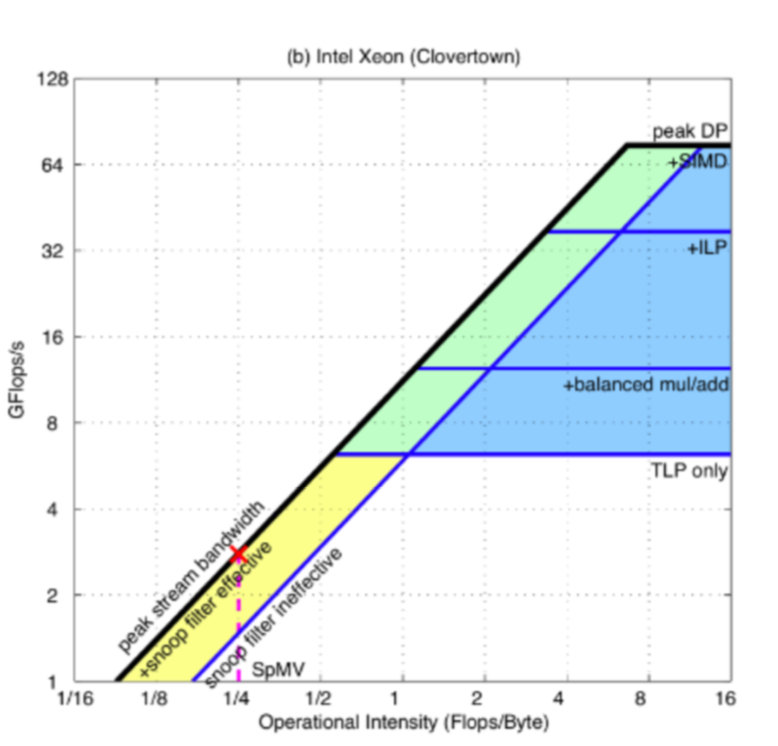
\includegraphics[width=10cm, height=8cm]{roof_example}

\section{Eigen}

Our main goal is to see how our code measures against Eigen code. 
Eigen is a library written in C++ which provides algorithms for fast matrix algebra, such as: dense and sparse product of matrix and vectors, matrix decomposition, space transformations. 


\section{LIKWID} 
One of the main tool is "likwid-perfctr", that offers access to hardware performance counters and derives metrics from the raw counts. 
By running likwid-perfctr, we can profile our code. The following screenshot is an example of an output: 

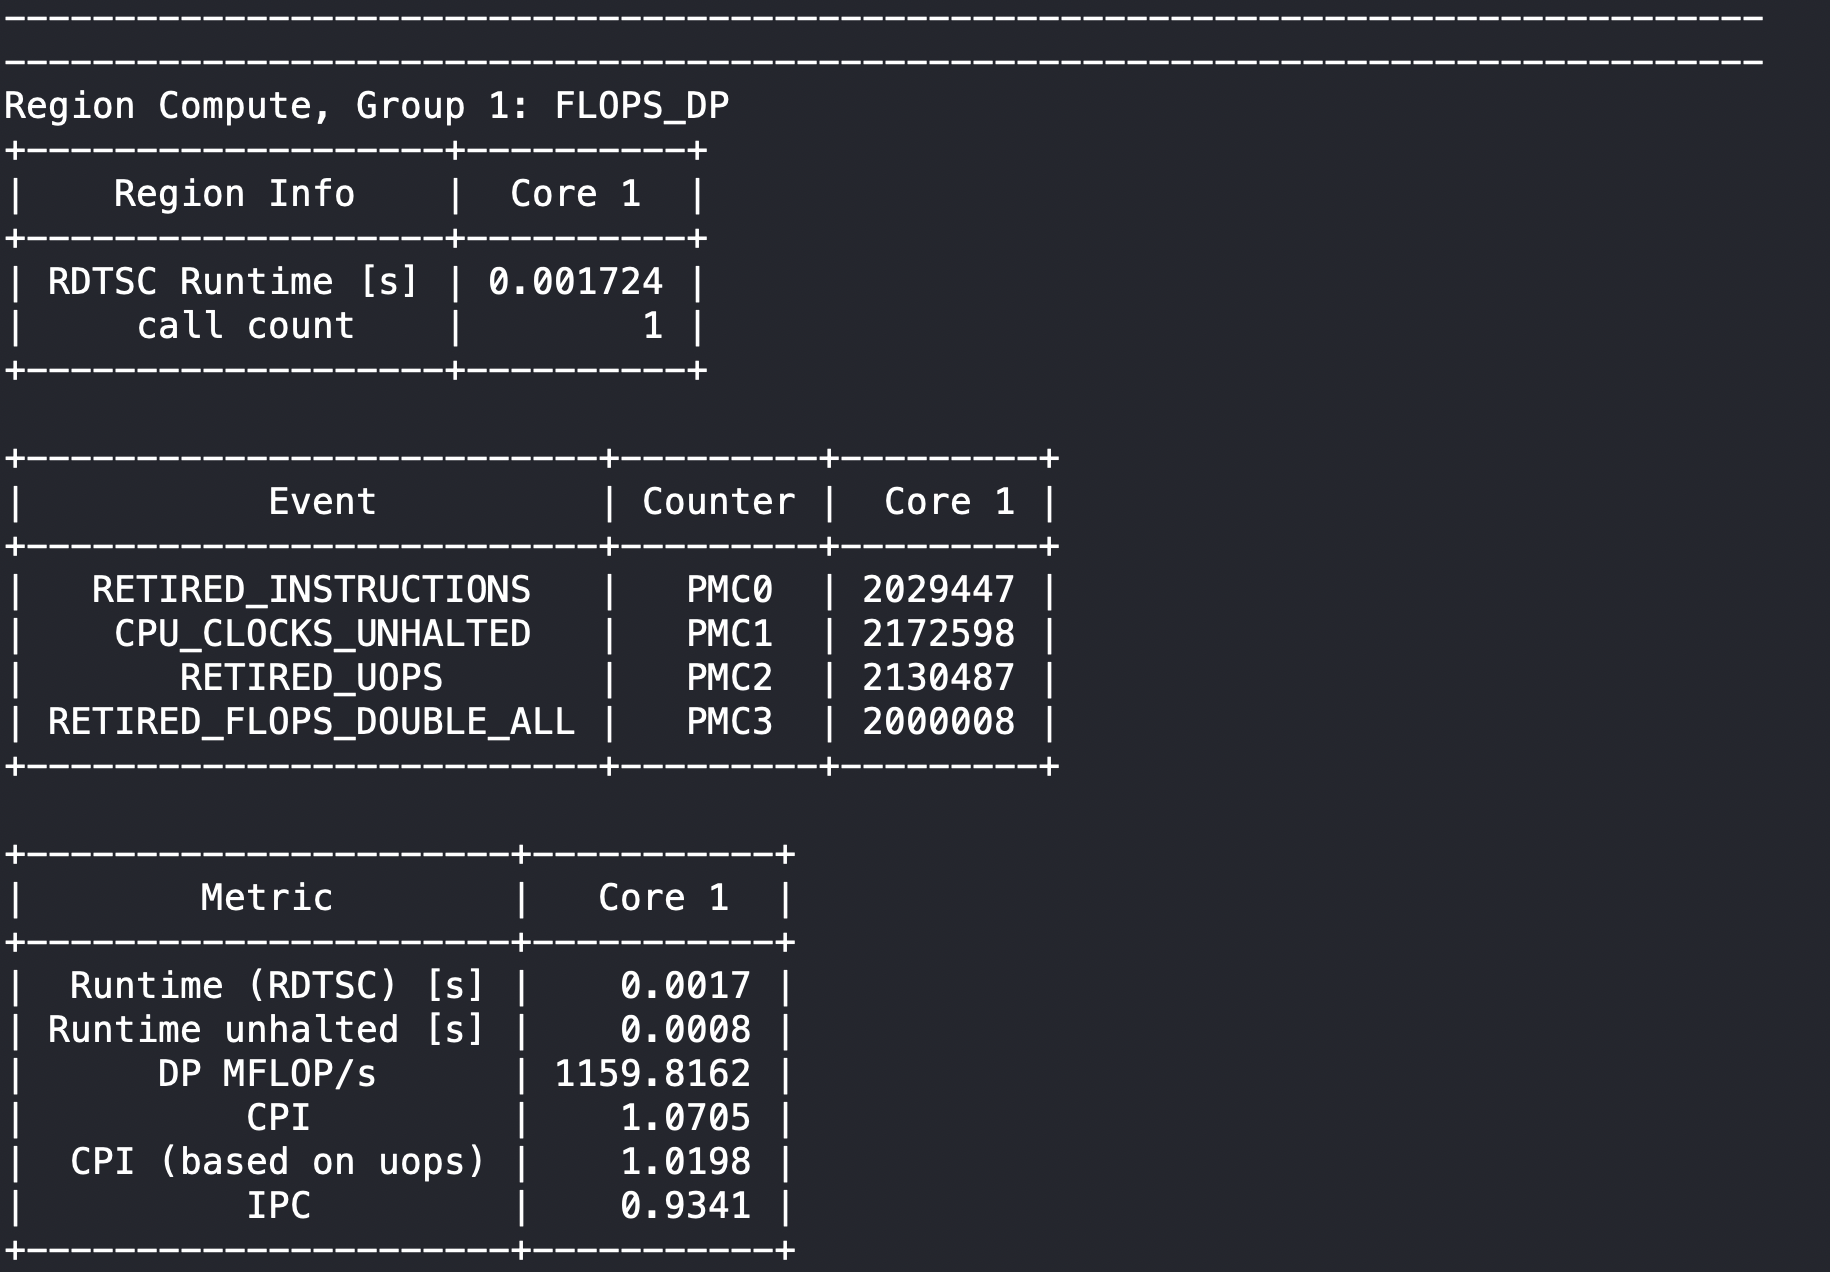
\includegraphics[width=10cm, height=8cm]{scree_lik_perf}

A brief explanation of all the metrics: 

\begin{itemize}
\item{\textbf{RETIRED\_INSTRUCTIONS}: instructions completely executed between two clocktick event samples.}
\item{\textbf{CPU\_CLOCKS\_UNHALTED}: number of cycles where CPU was not halted.}
\item{\textbf{RETIRED\_UOPS}: number of low-level hardware operations.}
\item{\textbf{RETIRED\_FLOPS\_DOUBLE\_ALL}: number of completely executed floating point operation per second  }
\item{\textbf{Runtime (RDTSC) [s]}: counts the number of cycles since reset. }
\item{\textbf{Runtime unhalted [s]}: counts the number of cycles since reset when CPU was not halted.}
\item{\textbf{DP MFLOP/s}:  number of double precision MFLOP/s.}
\item{\textbf{ CPI}: number of cycles per instruction retired.}
\item{\textbf{CPI (based on uops)}: Calculation of CPI based on uops.}
\item{\textbf{ IPC }: number of instructions per cycles}

Below some useful formulas that provide more insights into how these numbers are related to each other: 
\begin{itemize}
\item DP MFLOP/s = 1.0E-06*(RETIRED\_FLOPS\_DOUBLE\_ALL)/time
\item CPI = CPU\_CLOCKS\_UNHALTED/RETIRED\_INSTRUCTIONS
\item CPI (based on uops) = CPU\_CLOCKS\_UNHALTED/RETIRED\_UOPS
\item IPC = RETIRED\_INSTRUCTIONS/CPU\_CLOCKS\_UNHALTED


\end{itemize}

\end{itemize}


%%CAPITOLO 2
\chapter{Naive implementation}
At first we started with the simplest thing one could think of:
\lstinputlisting{naive_without_tmp.c}

In this case: blablabla calcoli su $P_peak$ computational intesity e grafico 

\chapter{Using a temporary variable to speed up cache lookup}

\chapter{Loop unrolling to exploit sum and multiplication pipelines}

\chapter{Parallel computations}

%%BIBLIOGRAPHY
\begin{thebibliography}{1}
\bibitem{likwid} 
Jan Treibig, Georg Hager, Gerhard Wellein, \textit{LIKWID: A lightweight performance-oriented tool suite for x86 multicore environments}. 
\bibitem{openmp}
Mark bull, \textit{A Short Introduction to OpenMP}
\bibitem{eigen}
Ga\"{e}l Guennebaud, Beno\^{i}t Jacob, \textit{Eigen v3}
\bibitem{roofmodel}
Samuel Williams, Andrew Waterman, David Patterson, \textit{An insightful visual performance model for floating point programs and multicore architectures}
\end{thebibliography}
 
 
 
 
 
\end{document}




